\documentclass[12pt]{jarticle} % Japanese
%\documentclass[12pt]{article} % English
% if there are problems in the above regarding fonts, use this
% \documentclass[UTF8]{ctexart}



%package
\usepackage{amssymb, amsmath, newtxmath}
\usepackage{cite}
\usepackage[utf8]{inputenc}
%\usepackage{utf}
\usepackage{naist-jmthesis} %Japanese
%\usepackage{naist-mthesis} %English
\usepackage[dvipdfmx]{graphicx}
\usepackage[dvipdfmx]{hyperref}
\usepackage{pxjahyper} %Required pxjahyper.sty
\usepackage[dvipdfmx]{xcolor}
\usepackage{pxjahyper} %TOC文字化け対策
\usepackage{booktabs}
\usepackage{here}



%definition
\definecolor{purple}{RGB}{98, 114, 164}
\hypersetup{
 colorlinks=true,
 linkcolor=black,
 citecolor=purple,
 urlcolor=black,
 filecolor=purple,
 anchorcolor=purple,
 pdfborder={0, 0, 1},
 linktoc=all
}
\renewcommand\thefootnote{\textcolor{purple}{\Roman{footnote}}}


% Page style
\pagestyle{final}       % Camera-Ready
%\pagestyle{draft}      % Draft
\lang{Japanese} % Japanese
%\lang{English} % English
% Student Number
\studentnumber{1811147}
\doctitle{\mastersthesis}% 修士論文
\major{\engineering}     % 工学



% 日本語題目 (in LaTeX)
\title{トンネリング抑止を目的とした\\分散ハッシュテーブルを利用したDNSに関する研究}
% 日本語題目 (in plain text)
%   注: (in LaTeX)と同じ場合は指定する必要なし。
%       この情報は修士論文/課題研究には現れませんが、管理のために必要です。
%\ptitle{再帰問い合わせ名前解決へのハッシュ関数を用いたDNS Exfiltration緩和策の提案}



% 英語題目 (in LaTeX)
%\etitle{Proposal for Mitigation of DNS Exfiltraion using Hash Function to Recursive Name Resolution}
\etitle{A Study of Domain Name System using Distributed Hash Table \\for Tunneling Deterrence}
% 英語題目 (in plain text)
%   注: (in LaTeX)と同じ場合は指定する必要なし。
%       この情報は修士論文/課題研究には現れませんが、管理のために必要です。
%\eptitle{Theoretical Studies on Low-Speed Calculation Algorithms of pi \\
%Utilizing the Sun and the Moon}
%\eptitle{Proposal for Mitigation of DNS Exfiltraion using Hash Function to Recursive Name Resolution}



% 日本語氏名 (in LaTeX)
%   (姓と名の間に空白を入れて下さい)
\author{高須賀 昌烈}
%\pauthor{}
%   (first name, last name の順に記入し、先頭文字のみを大文字にする。)
\eauthor{Shoretsu Takasuka}
% 別の例: \eauthor{Kurt G\"{o}del}
%\epauthor{}



% 論文提出年月日
\syear{2020}
\smonth{1}
\sday{28}



% 専攻の選択
%\department{\infproc}  % 情報処理学
%\department{\infsys}    % 情報システム学
%\department{\bioinf}   % 情報生命科学
\department{\infsci}    % 情報科学



% 審査委員(日本語)
%   (姓と名、名と称号の間に空白を入れて下さい)
%5人以上の場合,5人目以降は\addcmembers を使って宣言する。
%最大で合わせて8人まで宣言可能。
%主指導教員、副指導教員を明記する。両指導教員以外は委員。
%学外審査委員は、大学名を明記する
% 4人の場合
\cmembers{門林 雄基 教授}{(主指導教員)}
         {笠原 正治 教授}{(副指導教員)}
         {林 優一 教授}{(副指導教員)}
         {妙中 雄三 准教授}{(副指導教員)}
% 3人の場合
%\cmembers{○○ ○○ 教授}{(主指導教員)}
%         {○○ ○○ 教授}{(副指導教員)}
%         {○○ ○○ 准教授}{(副指導教員)}
%         {}{}
% 2人の場合
%\cmembers{○○ ○○ 教授}{(主指導教員)}
%         {○○ ○○ 教授}{(副指導教員)}
%          {}{}
%          {}{}



% 審査委員(英語)
%     (first name, last name の順に記入し、先頭文字のみを大文字にする。
%       first name と last name の間に空白、
%       last name と 称号の間にカンマと空白を入れて下さい。)
% 5人以上の場合,5人目以降は\eaddcmembers を使って宣言する
% Supervisor, Co-supervisor, and Member must be specified.
% 4人の場合
\ecmembers{Professor Youki Kadobayashi}{(Supervisor)}
          {Professor Shoji Kasahara}{(Co-supervisor)}
          {Professor Yu-ichi Hayashi}{(Co-supervisor)}
          {Associate Professor Yuzo Taenaka}{(Co-supervisor)}
% 3人の場合
%\ecmembers{Professor xx xx}{(Supervisor)}
%          {Professor xx xx}{(Co-supervisor)}
%          {Associate Professor xx xx}{(Co-supervisor)}
%          {}{}
% 2人の場合
% \ecmembers{Professor xx xx}{(Supervisor)}
%           {Professor xx xx}{(Co-supervisor)}
%           {}{}
%           {}{}



% ===================キーワード===================
\keywords{ドメインネームシステム,DNSトンネリング,分散ハッシュテーブル,P2Pネットワーク}
% キーワード5〜6個 (in plain text)
%   注: (in LaTeX)と同じ場合は記入する必要なし。
%       この情報は修士論文/課題研究には現れませんが、管理のために必要です。
%\pkeywords{pi, 天文学, 数学, 計算機, アルゴリズム}
%\pkeywords{DNS Exfiltration, 秘匿通信,ハッシュ関数,再帰問い合わせ}
% 5 or 6 Keywords (in LaTeX)
%\ekeywords{$\pi$, astronomy, mathematics, computer, algorithm}



% ===================Keyword===================
\ekeywords{Domain Name System(DNS), DNS Tunneling, Distributed Hash Table(DHT), P2P Network}
% 5 or 6 Keywords (in plain text)
%   注: (in LaTeX)と同じ場合は記入する必要なし。
%       この情報は修士論文/課題研究には現れませんが、管理のために必要です。
%\epkeywords{pi, astronomy, mathematics, computer, algorithm}
%\epkeywords{DNS Exfiltration, Covert Channel, Hash Function, Recursive Name Resolution}



% ===================内容梗概===================
\abstract{
% ネットワークプロトコルスタックの一つとして,IPアドレスとドメイン名を対応づけるDNSがある.
% 名前解決の機能を提供するDNSだが,情報流出として機能することが
}
%   注: 行の先頭が\\で始まらないようにすること。
%   注: (in LaTeX)と同じ場合は記入する必要なし。
%       この情報は修士論文/課題研究には現れませんが、管理のために必要です。
%       改行する箇所には空白行を入れる。
%       行の先頭が\\で始まらないようにすること。
%\pabstract{
%}
% Abstract (in LaTeX)
%  注:  行の先頭が\\で始まらないようにすること。



% ===================Abstruct===================
\eabstract{
}
% Abstract (in plain text)
%   注: (in LaTeX)と同じ場合は記入する必要なし。
%       この情報は修士論文/課題研究には現れませんが、管理のために必要です。
%       改行する箇所には空白行を入れる。
%       行の先頭が\\で始まらないようにすること。
%\epabstract{
%The calculation of pi has been paid much attention since human beings
%appeared on the earth.
%This thesis presents novel low-speed algorithms to calculate
%pi utilizing the sun and the moon.
%This is a sample abstract. This is a sample abstract.
%}



% ===================表紙===================
\begin{document}
\titlepage
\cmemberspage
\firstabstract
\secondabstract



% ===================目次===================
\toc
\newpage
\listoffigures
%\newpage
\listoftables



% ===================本文===================
\newpage
\pagenumbering{arabic}

\section{序論}
\subsection{背景}
ドメインネームシステム(Domain Name System, DNS)は,ドメイン名(E.g. www.example.com)をインターネット上でのノードの住所を表すIPアドレス(E.g. 93.184.216.34)に変換する機能を担っており,DNSを通じて特定した宛先に問い合わせることで我々はサービスにアクセスできている.
現在のインターネットの利活用において,名前解決の仕組みは極めて重要な技術の一つである.
しかし,性善説的な当時の設計に伴い生じた脆弱性を利用した攻撃がいくつか報告されている.
1987年にRFC1034, RFC1035(\cite{rfc1034, rfc1035})として公開されたDNSのコンセプトは,現在もなお本質的な仕組みは変更されることなく適用されている.
%近年では,平文であるDNSクエリを解析することでユーザがどのwebページを閲覧しようとしているのか,どこにメールを送信しようとしているのかといったユーザのプライバシーを侵害される脅威\cite{rfc7626}に関心が集まっており,HTTPSやTLSによってクエリおよび応答パケットを暗号化するDoH/DoTが盛んに議論されている.
その設計に起因する課題の内,DNSクエリのラベルおよびリソースレコード(Resource Record, RR)をデータ転送のメディアとするDNS Tunnelingがある.

DNS Tunnelingは,一般にフィルタリングされることが少ないDNSの特徴とDNSがデータ転送のメディアとして機能しているとは想像しない人の認知の隙間をついた手法であり,ファイヤー・ウォールやIDS/IPSといったセキュリティラインを突破するために使用される.
このように本来の目的とは違う方法でデータを転送する手法は,一般に秘匿通信(Covert Channel)と呼ばれる\cite{covertchannel}.
DNS Tunnelingは,秘匿通信の代表例であり,マルウェアとC2(Command \& Control)サーバとの通信の秘匿手法,または,ターゲットから取得したデータを外部に流出させるといった目的実行の手段として,実際のインシデントで広く利用されている\cite{frameworkpos, bondupdater, bernhardpos, multigrainpos, pisloader, denis, dnsmessenger, udpos}.
%2014年には,発生した大規模なクレジットカード情報流出事件\cite{},最近では2019年に発生したAPTグループ(通称,OilRig)による中東政府を標的とするサイバー攻撃のC2通信\cite{bondupdater}として実際のインシデントなどがある.
%このDNS Tunnelingのメカニズムは,スタブリゾルバからリカーシブサーバを経由し権威サーバへ問い合わせる一連の正規の仕組みに基づいており,名前解決を実現するにあたり生じる設計上の脆弱性を突いた手法である.
従来のDNS Tunnnlingに対するアプローチには,検知による手法が採用されてきた.
DNS TunnelingによるDNSクエリは,以下(\ref{eq:sample_qname})に示すように,転送量に比例して長いラベルを持ち,ラベルとしての文字列制約を満たすためのエンコーディングによって高いエントロピーを示す特徴がある.

\begin{eqnarray}
 \label{eq:sample_qname}
 \begin{aligned}
  &obqxg43xmqytcmjr.exfil.com\\
  &base32(password1111) = obqxg43xmqytcmjr
 \end{aligned}
\end{eqnarray}

また,インタラクティブなシェルなど双方向の通信をDNS Tunnelingで実現しようとする場合,時間あたりに高頻度なトラフィックが発生するという特徴が現れる.
このような特徴に基づき,パターンマッチングや機械学習,文字列分布などのメソッドを用いた検知手法が過去に多数考案されてきた\cite{born, cheng, liu, asaf, steadman, jawad}.
それら検知手法は,かなり高い精度で分類を実現しているものがあるが,DNS Tunnelingとして検知する対象としているパケットには一般に利用することができるDNS Tunnelingツールキット\cite{ozymandns, iodine, dnscat2}が使用され,それらは特に過剰な特徴量を示し,明らかに正規のDNSクエリと異なる特徴がある.
高い精度を示す従来の検知手法だが,しかし,それらを迂回する手法として,1回あたりの転送データ量を少なくすることで特徴量を減らすLow Throughputなバイパス手法,また,パケット間のインターバルを数日・数ヶ月と長期化させることでファイル肥大から一定期間しか保存されることがないログ管理の隙間を突いたSlowなTunenling手法があり,従来の検知手法では対応することが困難である.
悪意を持つユーザの視点として,1bitでも転送できることは秘匿通信として利用することができるため,転送量の少なさは軽視されるべきではない.

他方で,DNSは初めに述べたように,現在のインターネットの根幹技術として根ざしており,抜本的な改変は期待されない.
すなわち,既存のDNSによる名前解決のメカニズムに大幅な改変を加えないという制約下で,Tunnelingに対処することが現実的な最適解であると考える.


\subsection{目的}
本研究では,既存のDNSの名前解決メカニズムの大部分を流用することが一部の改変に留めながら,DNSを用いたデータ転送としての機能の排除を実現する次世代の名前解決メカニズムを提案する.
%\subsection{貢献点}
%本研究の貢献は,以下の通りである.
%\begin{itemize}
% \item 侵入通信を目的とするDNS Tunnelingに対するリアルタイム検知アルゴリズムの提案
% \item 既存対策アプローチとDNSの潜在的データ転送脅威モデルの検討
%\end{itemize}
%\subsubsection{脅威モデル}
%\subsubsection{仮説}




\subsection{本論構成}
%\ref{kako}節では、過去における研究について述べ、
%\ref{kadai}章では、現状と今後の課題について述べる。
%また、付録\ref{omake1}におまけその1を添付する。
本稿の構成は以下の通りである.
まず第2章で,準備として,DNSプロトコル・秘匿通信・Tunnelingメカニズム・分散データベースの4点について説明する.
第3章では,関連研究としてトラフィックおよびペイロード特徴に基づいた検知手法を説明し,それら手法がLow Throughput手法・Slow Tunneling手法に対して検知が困難であることを説明する.
第4章で提案手法とその実装について述べ,第5章で提案手法の性能評価と考察行い,第6章で残留する脅威モデルについて議論する.
最後に,第7章で結論と今後の課題について述べていく構成になっている.

\section{準備}
本章は第3章以降の要素補足を目的に,本論において核となる技術内容・特徴およびそのメカニズムについて説明する.
\subsection{DNS プロトコル概要}
\label{sec:dns-protocol}
DNS(Domain Name System)は,インターネットに接続された無数のコンピュータを一意に識別するためのIPアドレスを,人が認識しやすいドメイン名に変換するシステムである.
元来,インターネット上でのホストの識別にはIPアドレスが使用されてきた.
しかし,32bitの名前空間で10進数表記のIPv4(E.g. ``192.168.0.1"),もしくは,128bitの名前空間で16進数表記のIPv6(E.g. ``2001:200:16a:8::230")は,人にとって認識しにくいものである.
そのため,自然言語のようにアルファベットや数字で表記する方法が取られ,当初はその対応表であるhosts.txtが中央集権的に管理されていたが,やがてホスト数の増大に伴い管理が困難になっていき,提案されたのが対応表を分散的に管理するDNSである.

DNSのシステムアーキテクチャは,クライアント・サーバ構成で成り立っている.
一般に,クライアントがドメインを問い合わせた場合,サーバはドメインに対応づけているIPアドレスを応答することで,クライアントはドメインに対応づけられたIPアドレスを解決することができる.
ドメインからIPアドレスの解決は正引きと呼ばれ,IPアドレスからドメインの解決を逆引きと呼ぶ.

ドメインは,数字とアルファベットおよびハイフン(``-")の文字列で表記され,最大長は63オクテットと定義されている.
また,ドメインはルートを頂点とする階層構造をとり,各階層にはドメインを管理する主体が存在し,管理主体を委譲することによって分散的にデータベースを管理する仕組みを取っている.

\begin{figure}[h]
 \centering
 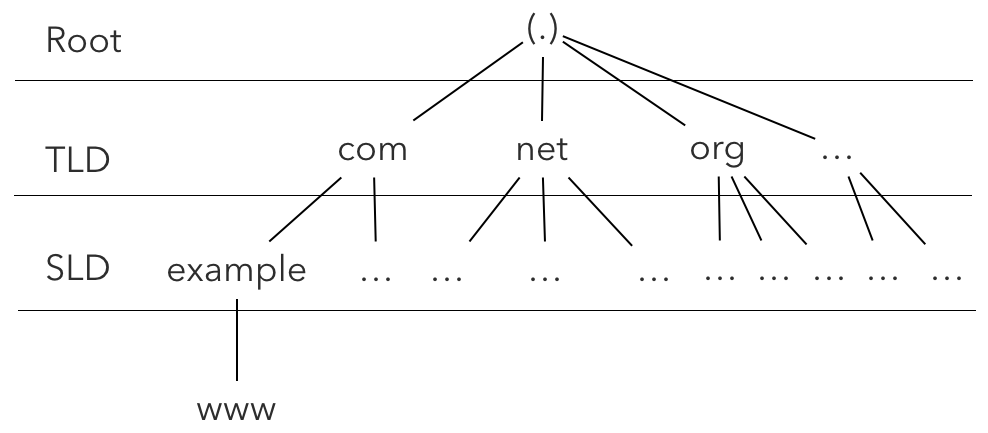
\includegraphics[width=12.0cm]{figure/dns-architecture.png}
 \caption{ドメインにおける名前空間}
 \label{fig:dns-architecture}
\end{figure}

ドメイン名は,ドメインに相当するラベルをドット区切りで表され,最大長は255オクテットである.
ドメイン名は右から順に階層序列が表現され,ドットで表現されるルートは一般には省略される.
最も右に位置づくラベルがTLD(Top Level Domain)であり,そのTLDからn番目(n $\mid$ n $\in$ $\mathbb{N}$)のラベルが第 n レベルドメインである.

TLDを大別すると,``.com"や``.net"をはじめとした特定分野別のgTLD(global Top Level Domain),``.jp"や``.ch"のような国ごとに割り当てられているccTLD(Co\\untry Code Top Level Domain)の二つに分けられる.
%TLDごとに登録するプロセスや必要書類,金額は異なり,上いの

\subsubsection{ノードの種類}
DNSは,機能に応じて3つに分類することができる.

\subsubsection{リソースレコード}
DNSの仕組みにおいて,ドメイン名に関連づけられた情報は,IPアドレス以外にも様々なものがあり,それらはリソースレコード(Resorce Record, RR)と呼ばれる.
DNSの仕組みによって,権威サーバが提供できる情報はドメイン名とIPアドレスの対応情報だけではない.
最も一般的なレコードは,Aレコードであり,FQDNをIPv4アドレスにマッピングする.
権威は,サブドメインへ委譲することが可能である.この機能は,NSレコードによって実現される.

\subsection{DNS Tunneling}
\label{sec:dns-tunnel}
DNSを利用して情報を外部に転送するには,初めにデータの宛先となるドメイン(E.g. exfil.com)を作成することになる.
転送する際のキャリアとなるDNSクエリのラベルには,使用できる文字列は数字・アルファベット・ハイフン(``-")である必要があるため,一般にBase32・64を用いて転送したい情報をエンコーディングすることでこの制約条件を満たす.
用意できたQNAME(E.g. arbitrary-string.exfil.com)について,例えばAのリソースレコードをクエリすると,サブドメインの存在の有無に関わらず,宛先となるドメイン(exfil.com)に任意の情報を転送することができるという具合である.
以下\ref{fig:dns-exfiltration}に,DNS Exfiltrationのメカニズムについて図解する.

\begin{figure}[h]
 \centering
 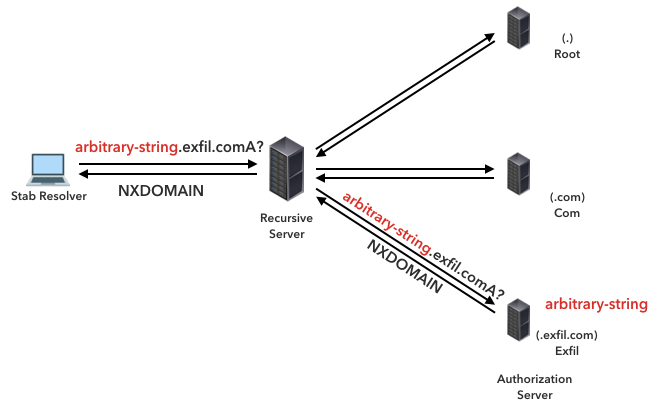
\includegraphics[width=12.0cm]{figure/dns-exfiltration.png}
 \caption{arbitrary-stringという任意の文字列が,DNSクエリのラベル部を用いて,事前に用意した権威サーバ(exfil.com)に転送される様子.}
 \label{fig:dns-exfiltration}
\end{figure}

また,管理する権威サーバのドメインに適当なホスト名(E.g. www)を作成し,そのホスト名のリソースレコード(E.g. TXT)に情報を付与していた場合には,そのホストへの問い合わせを通じて逆方向,すなわち権威サーバから任意の情報を転送することができる.
DNSのリソースレコードを転送キャリアとする流入通信のメカニズムを図解した様子が,\ref{fig:dns-tunneling}である.

\begin{figure}[h]
 \centering
 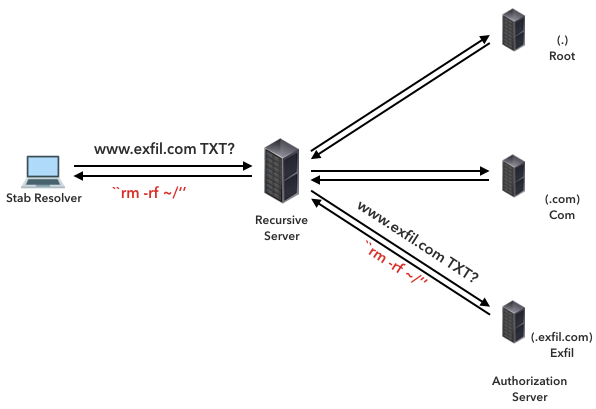
\includegraphics[width=10.0cm]{figure/dns-tunneling.png}
 \caption{事前にTXTレコードに登録された情報を問い合わせることで,権威サーバからの命令情報を取得している様子.}
 \label{fig:dns-tunneling}
\end{figure}

このようなDNSを用いて双方向な通信手法がDNS Tunnelingである.
%1998年4月,DNS Tunnelingの手法は,NmapのBugtraqメーリングリストにて初めて公になったとされている\cite{bugtraq}.


%\subsubsection{DNS Tunneling 特徴}
%%\subsubsection{その他課題}
%%\subsection{秘匿通信}
%%秘匿通信(英Covert Channel)とは,
%%情報転送を実現するにあたり,データの転送を本来の設計としていないプロトコルにそのデータを注入する手法である.
%%\subsubsection{ステガノグラフィ}
%%\subsubsection{代替プロトコル}
%\subsection{分散ハッシュテーブル}
%\subsubsection{アルゴリズム}
%\subsubsection{暗号学的ハッシュ関数}
%\subsection{P2P}
%\subsubsection{アーキテクチャ}

\section{関連研究}
\label{sec:related-works}
本章では,これまでに提案されてきたDNS Tunneling検知アプローチについてまとめ,1パケットあたりに転送データ量を少なくする手法とパケット間のインターバルを長期にする手法を用いることによって,バイパスできることを示す.
次に,これまでに提案されてきたP2Pベースの名前解決システムを説明し,提案手法との違いを述べる.
%最後に,既存の検知手法および次世代名前解決システムの課題から,既存のシステムに迎合しながらDNS Tunnelingを緩和する名前解決システムの必要性を明らかにする.

\subsection{特徴量に基づく検知手法}
本節では,DNS Tunnelingに対する先行研究のアプローチを紹介する.
\subsubsection{DNS Tunnelingにおける特徴量}
Bornら~\cite{born}は,ドメイン名に出現する文字の出現頻度を着目することで,正規のドメイン名とDNS Exfiltrationメソッドによって生成されたドメイン名とを分類のに有用であることを明らかにした(2010).
著者らは,正規のドメインであれば英語のような自然言語における文字の出現頻度と高い相関があることに加えて,エントロピーと文字列分布に高い相関があることも明らかにした.


\subsubsection{閾値推定}
\subsubsection{機械学習に基づくモデル}
%\subsubsection{パターンマッチング}
%\subsubsection{同一ドメインあたりのクエリ頻度}
%\subsubsection{Qnameにおける文字列分布}
%\subsubsection{Qnameにおける長さとエントロピー}
%\subsubsection{課題 : Low ThroughputなTunnelingに対する検知手法}
DNS Tunnelingメソッドを使用した時のDNSクエリは,第~\ref{sec:dns-tunneling}項で述べるような特性が出現する.
この性質に基づき,これまでに多数の検知手法が提案されてきた.


%\subsection{悪性DNS検知に関する研究}
\subsection{ポスト名前解決システム}
%また,新しいアーキテクチャを導入するとき 既存のシステムとのマイグレーションを考慮する必要がある点について,本提案手法がマイグレーションを考慮している設計である点について
\subsubsection{P2Pネットワークを利用した名前解決システム}
これまでに,DNSにおける〜の課題に対して,P2Pに基づいた名前解決システムは数多く提案されてきた.
\subsubsection{Blockchainを利用した名前解決システム}
%\subsubsection{フラットな名前空間に基づく名前解決システム}
\subsection{課題}
\label{sec:issue-past-works}
本節では,先行研究および新しいアーキテクチャに基づく名前解決システムにおけるDNS Tunnelingへの課題を示す.
(大筋)検知に基づく手法は,誤検知が避けられない.ペイロードアナリシスに対しては,一回あたりの転送量を調整することでバイパスすることができる.
分析の対象がトラフィックの場合は,頻度を長期間に延長することで,ログファイルの肥大によるストレージの過去のログファイルとの分析コストを重くなり分析の隙間をバイパスできる.
既存のアーキテクチャに基づくアプローチは,既存のDNSと根本から異なるアーキテクチャを採用しており,マイグレーションが考慮されていない.
また,ピュアのP2Pアーキテクチャおよびブロックチェーンのアーキテクチャでは,スタブリゾルバからのクエリが権威サーバとブロックチェーンをそれぞれ介することで,依然として,DNS Tunenlingとして機能し,発生を抑止するメソッドではない.

\section{提案システム}
本章では,DNSトンネリングの発生抑止を目的に設計した名前解決システムDNS-TD(DNS for Tunneling Deterrence)を説明する.
\begin{figure}[h]
 \centering
 \label{fig:abstruct-DNS-TD-architecture}
 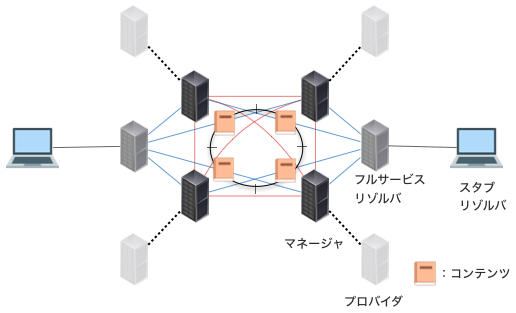
\includegraphics[scale=0.6]{figure/new-architecture-DNS-TD.png}
 \caption{提案システムの概略図}
\end{figure}
\subsection{概要}
\label{sec:DNS-TD}
現在のDNSの名前解決の仕組みにおいて,名前空間が委譲の仕組みに基づきドメインごとにゾーンで分割されているため,名前解決クエリは目的ドメインの権威サーバまで転送される必要がある.
また,リソースレコードはドメイン名に関係ない任意の情報を関連づけることができる設計になっている.
この2つの特性に起因して,DNSトンネリングは機能する.
すなわち,再帰問い合わせに基づく名前解決の仕組みとドメイン名に関連づけるレコード情報に高い自由度を排除することによって,DNSトンネリングの発生抑止を実現することができる.
一方で,名前解決システムとしての機能を維持するために,以下に示す2つの性質を満たす必要がある.
\begin{description}
 \item[名前解決]\mbox{}\\ ドメイン名にIPアドレスなどの情報を関連づけることができ,それを解決することができる
 \item[スケーラビリティ]\mbox{}\\ ドメイン名の増加および関連づけられるレコード情報の増加に対応することができる
\end{description}
%%設計要件
以上から,期待される名前解決システムの要件は,上記2つの性質を満たしながら先の特性を排除することである.
そこで,提案システムDNS-TDでは,不足が無視できる程度に大規模の名前空間と範囲に基づくゾーン分割によって名前解決とスケーラビリティを実現し,再帰問い合わせの特性を排除させ,認証システムによってリソースレコードの自由度を下げることで上記の要件を満たす.
以降では,その要件を満たすための手法および仕組みを概観する.\newline

\textbf{不足が無視できる程度に大規模の名前空間}\\
DNS-TDは,ドメイン名とレコード情報の組みには識別子を付与され,この識別子は672bit(84bytes)の有限名前空間上の一意に写像されたものを使用する.
識別子は,ドメイン名とそのレコードタイプの文字列和をメッセージとするハッシュ関数から算出されるダイジェストである.
例えば,ドメイン名が``www.example.com"でレコードタイプが``A"のペアを考える.
この場合,メッセージが``www.example.comA",識別子がこのメッセージをハッシュ関数に与えたダイジェスト``例:86ff(...中略...)8485"となる.\newline

\textbf{範囲に基づくゾーン分割}\\
識別子の名前空間について,ソートされた空間の特定範囲に基づいてゾーンが分割される.
提案システムにおけるサーバは,このようにして分割されたゾーンをそれぞれ担当することによって,分散的な管理システムとして協調することで名前解決機能を実現する.
提案システムにおけるサーバ機能は,一部を除いた\footnote{ccTLDとブランドTLDはSLDとして扱われ,それぞれ``cc"と``brand"というTLDに接続される.}gTLDによって集約される.
すなわち,SLD以降の権威サーバにサーバ機能はなく,ドメイン名とレコードタイプの作成と更新の機能のみを担う.
既存のSLD以降の権威サーバは,gTLDサーバにドメイン名の階層構造の序列を維持した状態で連結し,コンテンツ情報の操作を通じてgTLDにサーバ機能を委任する.
このように既存システムの権威サーバの機能を,サーバ機能とコンテンツ作成などの操作機能に分類することによって,クライアントからの権威サーバへの透過性を防ぎ,DNS Exfiltrationを抑止する.\newline

\textbf{認証システム}\\
DNS-TDでは,認証の仕組みを導入することでレコード情報の真正性を確保する設計をとっている.
既存システムでは,ドメイン名に関連づける情報はゾーンファイルにて定義されるが,ゾーンファイルを編集する主体が権威サーバであるため任意の情報を含めることができる設計になっている.
提案システムでは,先に述べるようにコンテンツの管理機能と編集機能とを分離させる.
コンテンツの編集機能は,サーバに階層的に接続されるノード,プロバイダが担う.
プロバイダを起点として行われるコンテンツへの操作は,認証機関を介在した後でサーバで実行される設計になっている.
この認証プロセスでは,依頼者(プロバイダ)情報およびレコード情報とその関連先となるドメイン名について真正性について検証される.
例えば,アドレスなどの情報であれば接続性が検証され,その他の情報であればレコード情報をドメイン名に関連づける正当性などが検証される.
この認証プロセスをパスし,証明書が発行されたコンテンツのみが,サーバによって管理される.
この認証プロセスによって,不審な情報がドメイン名に関連づけられることを未然に対処する.

以降では,上記3つのアプローチについて詳細に説明する.
また,DNS-TDで使う用語を表~\ref{tab:refres-terminology}にてまとめて示す.
\begin{table}[h]
 \centering
  \begin{tabular}{cl}
    \toprule
    \multicolumn{1}{c}{\textbf{表記}} & \multicolumn{1}{c}{\textbf{意味もしくは機能}}\\
    \midrule

    コンテンツ & \begin{tabular}{l}・識別子に関連づけられたレコード情報の実体\end{tabular}\\ \hline

    コンテンツID & \begin{tabular}{l}・識別子\end{tabular}\\ \hline

    レコード情報 &
      \begin{tabular}{l}
        ・リソースレコードの具体的な値\\
        (E.g. IPアドレス)
      \end{tabular}\\ \hline

     リソースレコードタイプ &
      \begin{tabular}{l}
        ・オブジェクトに関連づけるリソースレコードの型\\
        (E.g. A, AAAA, MX)
      \end{tabular}\\ \hline

    オブジェクト &
      \begin{tabular}{l}
       ・問い合わせる対象\\
       (E.g. ドメイン名もしくはIPアドレス)
      \end{tabular}\\ \hline

    スタブリゾル & \begin{tabular}{l}・名前解決クライアント\end{tabular}\\ \hline

    フルサービスリゾルバ &
      \begin{tabular}{l}
       ・スタブリゾルバからのクエリハンドリング\\
       ・識別子の作成
      \end{tabular}\\ \hline

    マネージャ &
      \begin{tabular}{l}
       ・フルサービスリゾルバからのクエリハンドリング\\
       ・ゾーンの管理\\
       ・コンテンツの保持
      \end{tabular}\\ \hline

    プロバイダ & \begin{tabular}{l}・コンテンツの作成・更新・削除操作\end{tabular}\\

    \bottomrule
  \end{tabular}
 \label{tab:refres-terminology}
 \caption{SORESにおける用語}
\end{table}



\newpage
\subsection{システムアーキテクチャ}
\label{sec:system-architecture}
本節では,DNS-TDのシステムアーキテクチャについて説明する.
現在,DNSはインターネットの根幹に位置づく技術であり,ほぼ全てのクライアントノードは既存システムが提供するアーキテクチャおよびプロトコルに依存している背景がある.
このため,システムのアーキテクチャの再構成において,エッジノードに対して変更が加えられるのは,導入負荷が高くなることが予想される.
現在のDNSによる名前解決は,フルサービスリゾルバを介在させながら,スタブリゾルバをクライアント,権威サーバをサーバとするクライアントサーバアーキテクチャで構成されている.
DNS-TDでは,導入フェーズで予想されるクライアントに対する名前解決処理システムの負荷を軽減することを目的として,従来同様のクライアントサーバアーキテクチャを踏襲する.
サーバ群は,図~\ref{fig:system-architecture}で示すように,相互で接続されたフルメッシュなネットワークで構築される.
\begin{figure}[htbp]
 \centering
 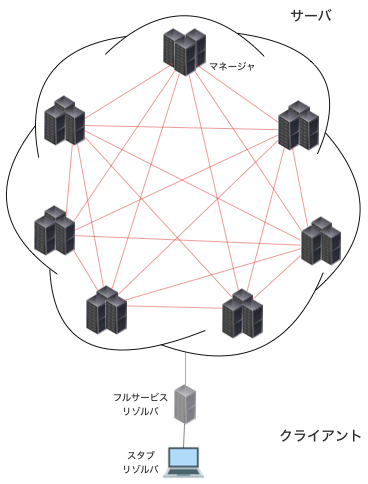
\includegraphics[scale=0.5]{figure/system-architecture.png}
 \caption{DNS-TDにおけるクライアントサーバアーキテクチャ}
 \label{fig:system-architecture}
\end{figure}
%クライアントからクエリは,フルサービスリゾルバを経由したのち
%コンテンツは,そのコンテンツIDとそのマネージャのゾーンを対応づけた対応表に基づいて一意に担当する
%各サーバは,コンテンツをそのコンテンツIDに基づいて分散的にかんりする
%クライアントからのクエリがあった際には
%コンテンツを分散的に管理しクライアントからのクエリに応答する.
%DNS-TDにおけるドメイン名の名前空間も既存システム同様に階層的な構造で構成されるが,サーバ

\subsection{サービスノード}
本節では,DNS-TDにおける各サービスノードの機能と他のサービスとの関わりについて詳細に説明する.
DNS-TDの名前解決ネットワークにおいて,クライアントがスタブリゾルバ,サーバの機能はマネージャが担当する.\newline

\hspace{-12pt}\textbf{スタブリゾルバ}\\
\label{sec:stab-resolver}
\hspace{12pt}スタブリゾルバは,既存システムと変わらない.
これは第~\ref{sec:system-architecture}節で述べるように,名前解決の仕組みの変化に伴ってクライアントに接続障害が発生する可能性がある.
既存のDNSに依存したクライアントの存在を踏まえて,接続性に影響を与えないためにスタブリゾルバは現行通りの方法で目的のリソース情報を解決することができる設計になっている.
すなわち,スタブリゾルバは,IPアドレスをはじめとしたオブジェクトに関連づけられたレコード情報を問い合わせ,目的サービスを提供するサーバのリソースにアクセスするクライアントノードである.
既存システム同様,スタブリゾルバのクエリはフルサービスリゾルバに転送され,キャッシュにヒットした場合には即座にレコード情報の応答結果を取得する.
ヒットしなかった場合には,フルサービスリゾルバがスタブリゾルバに変わって,サーバにクエリを転送し,応答結果をスタブリゾルバに返す.\newline

\hspace{-12pt}\textbf{マネージャ}\\
%具体的なTLDについてしっかりこのセクションで説明するべき
%マネージャの数
%プロバイダからの応答について説明するべきか
\hspace{12pt} マネージャは,2つの機能を担うサービスノードである.
それは,クライアントからの問い合わせに応答する機能と他のマネージャに操作リクエストを転送する機能である.
マネージャは,既存システムにおける権威サーバから分離した機能の一部であり,その残りの機能はプロバイダが担当している.
はじめに,マネージャとドメインおよびプロバイダの関係について説明する.

DNS-TDでは,既存のドメインの階層構造は引き継がれ,マネージャ・プロバイダそれぞれが独自のドメインを持っている.
プロバイダは,マネージャと親子関係にあるノードであり,マネージャが上位ドメイン,プロバイダが下位ドメインという構成である.
マネージャは,既存システムにおけるTLDに相当するドメインを保持する.
現在,TLDには国や地域に割り当てられるccTLDと分野別のgTLDの2つに大別することができる.
DNS-TDでは,コンテンツはそのIDに基づき管理する主体が決定する.
このため,ccTLDがマネージャである場合,国家間が抱えるナショナリズムや政治に起因して,名前解決システムの全体の運用に支障を来す事態が発生する可能性がある.
このことを回避するために,DNS-TDの設計ではマネージャが保有できるTLDをgTLDに限定している.
ccTLDは,``country"をドメインに持つマネージャにサーバ機能を委譲し,プロバイダとしてレコード情報の操作を行うことで現在のTLDと同等の位置づけを保つ.
これは,ドメインが``jp.country"となるのではなく,サーバ機能を``country"をドメインに持つマネージャに委ねるということである.
他方で現在,gTLDにはコミュニティ以外に``google"をはじめとした企業TLDがある.
先の国や地域に基づくシナリオであったように,民間企業の勝手な判断でインターネット全体に影響が波及するような接続性の断絶は起きうる.
そこで,企業やブランドを表すTLDは,``brand"というドメインにもつマネージャにサーバ機能を委譲し,プロバイダとして存在を継続させる.
その他のクラスとして分類することが困難な``foo"といったTLDについては,``misc"というドメインを持つマネージャにサーバ機能を委譲させる.
このように,DNS-TDでは,ドメインの名前空間を継続しながら,サーバとしての機能を再定義する.

以上のことを踏まえて,マネージャの機能について説明する.
1つ目は,ドメイン名とそれに関連づけられたレコード情報を保持し,フルサービスリゾルバからの問い合わせに応答する機能である.
マネージャは,レコード情報を管理するためにデータベースを用いる.
マネージャが保持するコンテンツは,そのドメイン名とレコードタイプによって決まる.
必ずしも自身のドメインを含むコンテンツを保持するわけではない.
例えば,``www.example.com"のAレコードについて考える.
この組のコンテンツIDが``47d8(中略\footnote{224bitのハッシュ値を表す.})cb6"であるとする.
他方で,``com"マネージャのゾーンは,``a000(中略)000"から``bzzz(中略)zzz"を担当しているとする.
また,``org"マネージャが``4000(中略)000"から``5zzz(中略)zzz"を担当しているとする.
この時,``www.example.com"はcomというTLDをもつが``com"マネージャではなく,``org"マネージャが保持する.
このようにして,コンテンツの管理は,ドメインに基づいて管理されるのではなくコンテンツIDの値とハッシュ値の範囲に基づいて決まる.

\begin{table}[htb]
 \caption{マネージャが使用する関数と保持する情報}
 \centering
  \begin{tabular}{ll}
    \toprule
		\multicolumn{1}{c}{\textbf{表記}} & \multicolumn{1}{c}{\textbf{意味}} \\
    \midrule
		parser() & クエリパケットをデータ構造に分解する関数 \\
		db\_accesser() & データベースにクエリする関数 \\
		benigh\_responce() & 正常応答用のペイロードを作成する関数 \\
		error\_responce() & 不在応答用のペイロードを作成する関数 \\
		payload.pack() & パケットのDNSのデータ構造にパックする関数 \\
		sendto() & クライアントに結果を応答する関数 \\
		record\_value & レコード情報 \\
    \bottomrule
  \end{tabular}
 \label{tab:discription-manager}
\end{table}

\begin{algorithm}[htbp]
 \caption{マネージャにおける名前解決問い合わせ処理}
 \label{algo:query-process}
  \SetKwProg{Fn}{}{\string:}{}
  \SetKwFunction{Handler}{handler}
  \SetKwFunction{Parse}{parser}
  \SetKwFunction{Database}{db\_accesser}
  \SetKwFunction{Noerror}{generate\_packet}
  \SetKwFunction{Error}{generate\_errror}
 $\vspace{-0.3cm}$\;
 %Calculate the content'{}s content id and domain id\;
 \Fn{\Handler{query\_data}}{
	 $content\_id,\ qtype \leftarrow parser(query\_data)$\;
	 $record\_value \leftarrow db\_accesser(content\_id)$\;
	 \If{$value$}{
		 $payload \leftarrow benigh\_response(content\_id,\ qtype,\ ttl,\ record\_value) $\;
		}
		\Else{
		 $payload \leftarrow error\_response(content\_id,\ qtype)$\;
		 }
		$payload \leftarrow payload.pack()$\;
		$sendto(payload,\ client\_address)$\;
 }

%クエリのパース\;
% %Calculate the content'{}s content id and domain id\;
% \Fn{\Parse{data}}{
%   $payload = DNSRecord.parse(data)$\;
%	 $return \ {'packet\_id':payload[0], 'content\_id':payload[1], 'q\_type':payload[2]}$\;
% }
%
%
% $\vspace{-0.3cm}$\;
% %Find the manager who has zone includes the content id\;
% DBへアクセス\;
% \Fn{\Database{content\_id}}{
%	$return \ Redis("127.0.0.1", 6379).get(content\_id)$\;
% }
% $\vspace{-0.3cm}$\;
%
% %Query the content to the manager\;
% 応答パケットの作成\;
% \Fn{\Noerror{packet\_id, content\_id, q\_type, ttl, record}}{
%	$payload = DNSRecord(DNSHeader($\;
%				$qr=1, aa=1, ra=1,id=packet\_id, rcode=RCODE["NoError"]))$\;
%	$payload.add\_question(content\_id, q\_type)$\;
%	$payload.add\_answer(c\_id, ttl, record)$\;
%  $return \ payload$\;
% }
% $\vspace{-0.3cm}$\;
%
% %Transfer the answer to client\;
% エラー応答パケットの作成\;
% \Fn{\Error{packet\_id, content\_id, q\_type, ttl, record}}{
%	$payload = DNSRecord(DNSHeader($\;
%				 $qr=1, aa=1, ra=1,id=packet\_id, rcode=RCODE["NXDomain"]))$\;
%	$payload.add\_question(content\_id, q\_type)$\;
%  $return \ payload$\;
% }
\end{algorithm}

2つ目は,プロバイダからコンテンツに対するの操作リクエストを受け付け,コンテンツIDを算出し担当のマネージャに操作リクエストを転送する機能である.
フルサービスリゾルバから問い合わせが発生した際,はじめにアルゴリズム~\ref{algo:manager}で示すようにクエリパケットからコンテンツIDを取得する.
次に,レコード情報を取得するために,コンテンツIDをキーとしてデータベースから対応するコンテンツを探索する.
コンテンツの存在の有無に従い,存在した場合にはレコード情報が応答され,実在しなかった場合には不在として応答される.
\begin{algorithm}[p]
 \caption{マネージャにおけるコンテンツ操作問い合わせ処理}
 \label{algo:registration-handler}
  \SetKwProg{Fn}{}{\string:}{}
  \SetKwFunction{Handler}{handler}
  \SetKwFunction{Certify}{certify}
  \SetKwFunction{Calc}{calculate\_id}
  \SetKwFunction{Find}{find\_manager}
 $\vspace{-0.5cm}$\;
 プロバイダからのコンテンツ操作リクエストハンドリング\;
 %Calculate the content'{}s content id and domain id\;
 \Fn{\Handler{request\_data}}{
	 $data,\ provider\_addr \leftarrow parser(request\_data)$\;
	 $content\_id,\ domain\_id \leftarrow calculate\_id(data.object,\ data.rtype)$\;
	 $manager\_addr \leftarrow find\_manager(start, end, content\_id)$\;
	 $sendto(data, manager\_addr)$\;
 }
 $\vspace{-0.5cm}$\;
 %Calculate the content'{}s content id and domain id\;
 コンテンツIDとドメインIDの算出\;
 \Fn{\Calc{qname, rtype}}{
   $content\_id \leftarrow hash.sha3\_224(qname+rtype)$\;
   $domain\_id \leftarrow hash.sha3\_224(qname)\ /\ 2$\;
   $return \ content\_id,\ domain\_id$
 }
 $\vspace{-0.5cm}$\;
 %Find the manager who has zone includes the content id\;
 コンテンツIDが含まれるゾーンを保持するマネージャアドレスの解決\;
 \Fn{\Find{start, end, content\_id}}{
   \For {$i,\ j\ \textbf{in}\ map\_start,\ map\_end$} {
     \If {$i \leq content\_id \leq j$} {
       $p \leftarrow map\_start.index(i)$\;
       $manager\_addr \leftarrow map.addr[p]$\;
       $return\ manager\_addr$\;
     }
   }
 }
 $\vspace{-0.3cm}$\;
\end{algorithm}


\newpage
最後に,マネージャにおけるコンテンツの管理について説明する.
コンテンツの実態は,以下に示す4つの要素が含まれた情報の集合である.
\begin{itemize}
 \item ドメイン名
 \vspace{-3mm}
 \item レコードタイプ
 \vspace{-3mm}
 \item TTL(Time To Live)
 \vspace{-3mm}
 \item レコード情報
 \vspace{-3mm}
 \item 証明書
\end{itemize}
保持するコンテンツ情報は,上記で示すように,長さに変化のある固定数の文字列で表現される要素が単純に列挙された構造である.
このデータには,クエリ情報に基づいてデータリソースにアクセスできることがDNS-TDにおけるデータモデルの要件になる.
名前解決におけるクエリ情報は,ドメイン名とそれに関連づけるデータのタイプ情報であることから,この2つの情報に基づいて生成される識別子をキーとして,コンテンツをバリューとするKVSモデルが最も単純であると考えられる~\cite{Davoudian}.
以上のことを踏まえ,DNS-TDでは,図~\ref{fig:manager-provider}に示すように,クエリ情報から算出される識別子をキー,コンテンツ情報をカンマ区切りで表現した文字列で表現したデータをバリューとするモデルを採用する.
\begin{figure}[h]
 \centering
 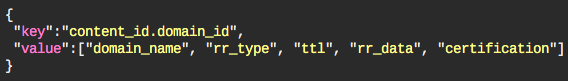
\includegraphics[scale=0.6]{figure/content-file.png}
 \caption{コンテンツのデータフォーマット}
 \label{fig:manager-provider}
\end{figure}

\hspace{-12pt}\textbf{フルサービスリゾルバ}\\
\hspace{12pt}フルサービスリゾルバは,サーバからの応答をキャッシュするを持つサービスノードである.
また,コンテンツIDおよびドメインIDを算出し,コンテンツを保持するマネージャに問い合わせる機能を担う.
全てのフルサービスリゾルバは,マネージャとそのマネージャのゾーンに関する対応表のファイルを保持している.
この対応表は,ICANNから提供される``Root.hints"ファイルのようにウェブ上で公開され,入手することができる.
フルサービスリゾルバは,アルゴリズム~\ref{algo:full-service}で示すように,スタブリゾルバからのクエリに含まれるドメイン名とレコードタイプに基づきコンテンツIDとドメインIDを導き出す.
コンテンツを保持するマネージャは,コンテンツIDが含まれるゾーンを探索することで一意に決定される.
名前解決には,``コンテンツID.ドメインID"のようにドット区切りでIDを組み合わせたものを識別子としてマネージャに問い合わせる.
レコード情報もしくは不在情報に関する応答パケットをマネージャから受け取ると,フルサービスリゾルバは既存システム同様に応答情報をキャッシュした後,スタブリゾルバに応答する.
\begin{table}[htb]
 \caption{フルサービスリゾルバが使用する関数と保持する情報}
 \centering
  \begin{tabular}{ll}
    \toprule
		\multicolumn{1}{c}{\textbf{表記}} & \multicolumn{1}{c}{\textbf{意味}} \\
    \midrule
		query\_manager() & マネージャに問い合わせる関数 \\
		response\_client() & 結果をクライアントに応答する関数 \\
		hash.sha3\_224() & 54bytesのSHA3ハッシュ関数 \\
    start & ゾーンにおける範囲の開始アドレス \\
    end & ゾーンにおける範囲の終了アドレス \\
    client\_address & クライアントのIPアドレスとポートのタプル \\
		answer.rcode & マネージャにおける応答コード \\
		answer.rdata & レコード情報 \\
    map\_start & ゾーンにおける範囲の開始アドレスのリスト \\
    map\_end & ゾーンにおける範囲の終了アドレスのリスト \\
    \bottomrule
  \end{tabular}
 \label{tab:discription-fullresolv}
\end{table}

\begin{algorithm}[htbp]
 \caption{フルサービスリゾルバにおける問い合わせ転送処理}
 \label{algo:full-service}
  \SetKwProg{Fn}{}{\string:}{}
  \SetKwFunction{Handle}{handler}
 $\vspace{-0.3cm}$\;
% クエリハンドリング\;
 \Fn{\Handle{query\_data,\ rtype}}{
   $content\_id,\ domain\_id \leftarrow calculate\_id(query\_data,\ rtype)$\;
	 $manager\_addr \leftarrow find\_manager(start,\ end,\ content\_id)$\;
	 $answer \leftarrow query\_manager(manager\_addr,\ content\_id,\ domain\_id)$\;
	 $response\_client(client\_address,\ qname,\ answer.rcode,\ answer.rdata)$\;
 }
 $\vspace{-0.3cm}$\;
\end{algorithm}


\newpage
\hspace{-12pt}\textbf{プロバイダ}\\
\hspace{12pt}プロバイダは,既存システムの権威サーバの機能のうち,レコード情報を操作する機能を担当するノードである.
すなわち,既存システムのSLD以降のドメイン情報に関して,作成・更新および消去といったレコード情報の操作を担当する.
メインの階層構造に上位のドメインを保持するマネージャが,プロバイダが保持するドメインのサーバ機能を担当する.
プロバイダは,認証局にてコンテンツ情報の真正性を評価されたのちに,プロバイダの上位に位置づくマネージャがそのコンテンツを担当するマネージャに依頼することでレコード情報を操作する.
プロバイダが認証局に転送する情報には以下の4つである.
\begin{itemize}
 \item ドメイン名
 \vspace{-3mm}
 \item レコードタイプ
 \vspace{-3mm}
 \item TTL(Time To Live)
 \vspace{-3mm}
 \item レコード情報
\end{itemize}
%%TTLの更新方法について説明する
%例えば,example.comプロバイダが``www"のIPアドレス情報を作成することを考える.
%example.comプロバイダは,``www.example.com"とレコードタイプ``A"およびその値``93.184.216.34"を含むデータを接続先のcomマネージャにリクエストする.
%comマネージャは,リクエストされたドメイン名とそれに関連づけるレコードタイプから識別子を算出し,担当のマネージャにストアリクエストを転送するという具合で動作する.

\newpage
\hspace{-12pt}\textbf{認証局}\\
\hspace{12pt}認証局は,レコード情報の真正性を検証する信頼された第3者機関である.
%目的から
DNSを用いた既存の名前解決システムでは,ドメイン名に任意の情報を関連づけることができることに起因して,DNSトンネリングとして利用される課題があった.
この課題に対してDNS-TDでは,ドメイン名に関連づけるレコード情報について,第3者機関からの認証を介在させることによって,不審な情報がドメイン名に関連づけられることを抑止する.
認証局を用いた認証プロセスでは,プロバイダからのドメイン名へのレコード情報を関連づけるリクエストをきっかけとする.
認証局に転送されるリクエストパケットについて,認証局は内容と依頼元の情報に基づいたデータの真正性を検証する.
この検証フェーズで認証されたコンテンツは,リクエストしたプロバイダの上位に位置づくマネージャに証明書を付与して転送される.
認証されなかった場合には,リクエストは破棄され,結果がリクエストしたプロバイダに応答される.

例えば,ドメイン名が``www.example.com"で,このドメイン名に``uname -ax"という文字列をTXTレコードに関連づけることを考える.
プロバイダは,認証局を宛先としてコンテンツの真正性に関する検証評価を依頼する.
依頼には,関連づける目的を合わせて要求する.
認証局は,関連づけたい内容と目的とを評価する.
この場合,``uname -ax"はLinuxコマンドであり不審なデータとして評価され,リクエストは破棄される.
関連づける情報が,IPアドレスであった場合には,接続性が評価された後,証明書を付与したコンテンツをマネージャに転送する.
これが認証における一連のプロセスであり,これによって不審なデータがドメインに関連づけられることを抑止する.
\begin{figure}[h]
 \centering
 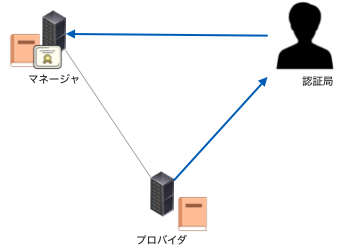
\includegraphics[scale=0.7]{figure/certificate-procedure.png}
 \caption{レコード情報操作におけるプロセスの概略図}
 \label{fig:manager-provider}
\end{figure}
% 認証局を導入するとインターネットの匿名性を実現することが難しくなるのではないか
% レコード情報に認証局を導入する場合,webなどのサービスやコンテンツを提供するのが少し困難になるではないかという懸念


\newpage
\subsection{識別子}
%ハッシュ空間によってIDが管理されることとどのハッシュ関数を使用するのかを説明する.
%ゾーンごとに分離される階層構造モデルに起因して発生するトンネリングに対して,フラットな名前構造が重要になる
本節では,コンテンツに付与する識別子について説明する.
DNSの名前解決システムでは,委譲の仕組みに基づいてドメインごとにゾーンを保持する設計のため,名前解決にあたりクエリ情報はそのドメイン名をゾーンとする権威サーバまで転送される.
この仕組みでは,ドメインを作成することで,そのドメインをゾーンにもつ権威サーバに対して任意の情報をDNSクエリに含めることでデータを転送することができる,DNSトンネリングとして機能する潜在的な特性がある.
転送する際に,正規のクエリ時に使用される長さや文字列に調整することで,正規クエリとトンネリングクエリを判別することは曖昧でき,このようにしてセキュリティシステムを迂回される脅威に発展する.
この課題は,名前空間を保持する機能とその空間上のドメイン情報を提供する機能が共在することに起因する.
そこで,DNS-TDでは,名前空間の保持機能と提供する機能を分離することで課題を解決する.
これは,ドメインの名前空間は維持したまま,コンテンツに識別子を付与し,この識別子の名前空間をフラットにすることで実現される.
DNS-TDでは,ドメイン名とレコードタイプという組みを単位として,全ての組みに画一的な名前空間上の値をその組みに識別子として付与する.
このように,DNS-TDでは,全てのドメイン名とレコードタイプの組みに識別子を付与するため,その識別子の名前空間は数の不足が無視できる程度に大きくなくてはならない.
また,~\ref{sec:stab-resolver}で述べるように,既存の名前解決の仕組みに依存したものは多く,プロトコルのフォーマットに変化を加えないことが望ましい.
DNSのクエリパケットにおいてデータを含められるQuestionセクションのQnameの最大長は,255bytesである.
また,Qnameはドメイン名を想定した設計になっているため,ドメイン名の制約にある最大63bytesとするラベル長の制約を満たす必要がある.
上記の制約を満たしながら,ドメイン名とレコードタイプから生成される識別子には,54bytesの名前空間を持つハッシュ関数によって生成されるメッセージダイジェストを用いる.
また,ダイジェストの衝突には,二重ハッシュ法に基づき対処する.
以降では,識別子に用いられるハッシュアルゴリズムとシステムの分散処理を目的としたゾーン分割法について説明する.

\subsubsection{ハッシュアルゴリズム}
本項では,コンテンツを識別するために使われる識別子の算出に利用するハッシュアルゴリズムについて説明する.
先に述べたように,提案システムで使用するハッシュアルゴリズムの要件は以下で示す通りである.
\begin{itemize}
 \item 不足を無視できる程度に大きい名前空間
 \vspace{-3mm}
 \item DNSプロトコルフォーマットへの準拠\\(ラベル長:最大63bytes,ドメイン長:最大253bytes)
\end{itemize}

%現在のインターネットにおいて,各権威サーバがゾーンを保持する設計のため,ドメイン名とレコードタイプの組みの数を正確に見積もることは困難である.
%ドメイン名の数は,インターネット上のサービスの数に相当すると考えることができ,そのドメイン名に関連づけられるリソースレコードの数は100も超えない数である.
%IPv6は全てのホストのインターフェースに一意に識別知を付与するのに,不足を無視できる名前空間として128bit(16bytes)を採用している.
%クライアントの数に比べて,サーバの数は少ないことは予想することができるが.その比率は不明である.
%そこで,現在使用できるハッシュアルゴリズムの特性から考える.
現在流布している代表的なハッシュアルゴリズムには,以下のようなものがある.
\begin{table}[htb]
 \caption{ハッシュアルゴリズムの一覧}
 \centering
  \begin{tabular}{lr}
    \toprule
		\multicolumn{1}{c}{\textbf{アルゴリズム}} & \multicolumn{1}{c}{\textbf{名前空間(bits)}} \\
    \midrule
		MD5 & 128 \\
		sha1 & 160 \\
		sha2 & 224,\ 256,\ 384,\ 512 \\
		sha3 & 224,\ 256,\ 384,\ 512 \\
    \bottomrule
  \end{tabular}
 \label{tab:hash-functions}
\end{table}

IPv6は全てのホストのインターフェースに一意に識別知を付与するのに,不足を無視できる名前空間として128bitsを採用している.
通常クライアント数の数に対してサーバの数は少なく,ドメイン名に関連づけられるリソースレコードの数はたかだか数から数十個である.
表~\ref{tab:hash-functions}で示すハッシュアルゴリズムの名前空間は,128bitsと同等かそれより大きい.
リソースレコードの数を含める
2のべき乗の桁数は,おおよそ$2^{0.301n}$$(n \in \mathbb{N})$から求めることできる.
で求めることができる.
これに基づき,160bitが

以上から,識別子として必要な名前空間は,128bitよりも少ない.
以上から,DNS-TDでは,最も出力長の短い56bytesの名前空間をもつsha3のアルゴリズムを採用する.

ハッシュ関数は有限空間に写像する性質から,写像したダイジェストが他のコンテンツによって算出されたダイジェストと衝突する可能性がある.
以降では,ダイジェストのコリジョンを回避するために,さらに名前空間は拡張するドメインIDについて説明する.
DNS-TDにおけるコンテンツIDは,ドメイン名とレコードタイプの文字列和をメッセージとするハッシュ関数のダイジェストである.

\begin{algorithm}[h]
 \caption{識別子の導出方法}
 \label{algo:calculate_id}
  \SetKwProg{Fn}{}{\string:}{}
  \SetKwFunction{Calc}{calculate\_id}
% $\vspace{-0.3cm}$\;
 \Fn{\Calc{qname, rtype}}{
   $content\_id \leftarrow hash.sha3\_224(qname+rtype)$\;
	 $domain\_id \leftarrow hash.sha3\_224(qname)[:28]$\;
	 $identity \leftarrow content\_id\ +\ ``."\ +\ domain\_id$\;
   $return \ identity$
 }
% $\vspace{-0.5cm}$\;
\end{algorithm}


例えば,ドメイン名が``www.example.com"でAのレコードタイプの組み合わせを考える.
アルゴリズム~\ref{algo:calculate_id}に従い,コンテンツIDのメッセージになるのは``www.example.comA"である.
そして,このメッセージをハッシュ関数にかけて算出された値``47d87[...中略...]4cb6"がコンテンツIDとなる.
ドメインIDは,ドメイン名をメッセージとするハッシュ関数から算出されるダイジェストの前半28bytesである.
すなわち,メッセージが``www.example.com"で,``86ff20[...中略...]bf026"がドメインIDとなる.
以上から,最終的なマネージャに問い合わせられる識別子は,それぞれのIDをドット区切りで連結された``(コンテンツID).(ドメインID)"となる.

\subsubsection{ゾーン分割}
本項では,ゾーンの分割方法とそのゾーンとマネージャの対応表について説明する.
DNS-TDにおけるゾーンは,ソートされたコンテンツIDの名前空間の連続した範囲に従って分割する.

\begin{table}[htb]
 \caption[マネージャとゾーンの対応表]{マネージャの情報とそのマネージャが管理するゾーンが記載された対応表の例}
 \centering
  \begin{tabular}{lrl}
    \toprule
		\multicolumn{1}{c}{\textbf{ゾーン}} & \begin{tabular}{c}\textbf{マネージャ}\\\textbf{アドレス}\end{tabular} & \multicolumn{1}{c}{\textbf{ドメイン}} \\
    \midrule
    (000…00, 2zz…zz) & 192.35.51.30 & com.  \\
		\multicolumn{1}{c}{...} & \multicolumn{1}{c}{...} & ... \\
    (500…00, 6zz…zz) & 192.5.6.30 & net. \\
		\multicolumn{1}{c}{...} & \multicolumn{1}{c}{...} & ... \\
    (b00…00, czz…zz) & 199.249.112.1 & org. \\
		\multicolumn{1}{c}{...} & \multicolumn{1}{c}{...} & ... \\
    (n00…00, mzz…zz) & 199.254.31.1 & info. \\
		\multicolumn{1}{c}{...} & \multicolumn{1}{c}{...} & ... \\
    (y00…00, zzz…zz) & 194.0.0.53 & arpa. \\
    \bottomrule
  \end{tabular}
 \label{tab:hash-management}
\end{table}


表~\ref{tab:hash-management}で示すように,``com"ドメインを管理するマネージャは``000...00"から``2xx...xx"の連続した範囲の名前空間を管理する.
コンテンツIDがこの範囲下に含まれる場合には,``com"に問い合わせることによってレコード情報を管理することができる.
対応表は,ICANNから提供される``Root.hints"ファイルのようにウェブ上で公開され,常時入手可能な状態が維持される.
全てのフルサービスリゾルバおよび認証局は,この対応表を保持することで,コンテンツIDを算出することで一意に管理するマネージャを特性することができる.

% 提案システムで使用するレコードタイプを概観するか,もしくは既存システムにおけるリソースレコードのタイプの課題から説明するのがいいだろう
\subsection{レコードタイプ}
本項では,DNS-TDで使用するリソースレコードのタイプについて説明する.
第~\ref{sec:dns-infiltration}項で示すように,既存の名前解決システムでドメインに関連づけることができるリソースレコードのいくつかのタイプは,DNS Infiltrationとして機能することができる.
DNS Infiltrationを抑止するリソースレコードであることの必要条件は,ドメインに関連のない任意の文字列がレコード情報に含められないことである.
既存のDNSのリソースレコードのタイプのうち,任意の文字列を含めることができるのタイプは以下の通りである.

表~\ref{tab:infil-rtype}のDNS Infiltrationとして機能する可能性のあるリソースレコードのタイプのうち,IPアドレスを偽装して情報を転送するものについては,第~\ref{sec:certificate}項で述べた認証基盤によってレコード情報の正当性評価で排除することができる.
NULL・TXT・CNAMEのレコードタイプも認証基盤における正当性の評価に基づいて,目的にそぐわない内容を含む場合には署名の作成を破棄することでDNS Infiltrationの発生を抑止する.

%特定のハッシュ範囲を管理するノードは,複数用意させ,そのアドレスを対応表に明記し,ストアする際にその全てのレプリケーションサーバにストアリクエストする
%DNSSEC~\cite{rfc4033}は,権威サーバからの応答パケットの偽装を検知することを目的として,データの作成元の確認とデータの完全性および,不在情報応答情報の証明するDNSの拡張仕様である.
%これは,主としてDNSの応答パケットを偽装できる程度のパラメータであることに起因する.
%他方で,DNS-TDでは,応答パケットに224bitのメッセージダイジェストが含まれるため,悪意のある応答パケットをフルサービスリゾルバに意図的にキャッシュすることは極めて困難である.以上の理由から,DNS-TDではDNSSECの目的にそぐわないため,リソースレコードとして使用されない.


\section{評価}
\subsection{実装}
\subsection{実験環境}
\subsection{DNS Tunnelingに対する理論評価}
\subsubsection{評価要素 : 対Exfiltration}
\subsubsection{評価要素 : 対Infiltration}
\subsection{シミュレーション実験に基づく特性評価}
\subsubsection{評価要素 : パケットサイズ}
\subsubsection{評価要素 : トラフィック量}
\subsubsection{評価要素 : RTT(Round Trip Time)}

\section{考察}
\subsection{マネージャノードの最適な数}
%\subsection{検閲}
%提案システムでは,ドメイン名とそれに関連付けれたレコード情報のペアに基づき構成されるコンテンツは,フラットな名前空間に一意にマップされる.
%コンテンツは,ソートされたハッシュ値の特定の範囲ごとに分割され,その範囲をゾーンとしてマネージャサービスによって管理される.

\subsection{コンテンツIDを計算する最適ノード}


\section{結論}
% 機能を分離させることによって,クエリを用いてデータを転送する仕組みを無効化することを実現
% 他の名前解決システムと違い,クライアントサイドへの変更点が少ないためマイグレーションが期待される
本論文では,DNSトンネリングを抑止する名前解決システムを提案した.
DNSトンネリングが動作する仕組みについて分析し,スタブリゾルバからコンテンツを操作する権威サーバまで問い合わせパケットが転送される点に着目した.
提案システムDNS-TDでは,権威サーバの機能をコンテンツを保持しクライアントからの問い合わせに応答する機能とコンテンツを編集する機能を2つサービスノードに分割させる.
この設計によって,スタブリゾルバからの問い合わせパケットを受信するノードを作成することが防ぐことで,トンネリング通信の発生を抑止する.
また,提案システムの機能特性について評価を行い,既存システムよりも少ないトラフィックでなおかつ高速な名前解決を実現できるという優位性を持っていることを示した.
DNSは現在のインターネットの根幹技術であり,基盤システムに根付いているため,既存システムから完全に移行することは困難である.
この点を踏まえて,提案システムでは,フルサービスリゾルバと権威サーバにおけるトランザクションのみの変更に抑えることで.既存システムからの移行を実現しやすいものに設計した.

今後の課題として,最適なマネージャノードの数を推定することがある.
これには,マネージャが保持するコンテンツの数とその計算負荷の関わりについて評価する必要がある.
また,現在のDNSのルート権威サーバに適用されるようなAnycast技術を用いることで,地理的制約を解消し少ないマネージャ数で運用できる可能性がある.
この課題について検討を行っていく.




% ===================謝辞===================
\newpage
\acknowledgements
ご指導ご鞭撻賜りありがとうございました.




% ===================参考文献===================
% ここでは \reference を使って、自分でリストを作るか、BibTeX を使って
% リストをつくって下さい。この例では BibTeX を作るような形式になってい
% ます。
\newpage
%\reference
%\bibliographystyle{plain}
\begin{thebibliography} {25}\small
 \bibitem{rfc1034} P.V. Mockapetris. ``Domain names - concepts and facilities. RFC 1034 (INTERNET STANDARD)," November 1987.
 \bibitem{rfc1035} P.V. Mockapetris. ``Domain names - implementation and specification. RFC 1035 (INTERNET STANDARD)," November 1987.
 \bibitem{rfc4033} R. Arends, R. Austein, M. Larson, D. Massey, S. Rose. ``DNS Security Introduction and Requirements, " March 2005. Updated by RFCs 6014, 6840.
 \bibitem{rfc4648} S. Josefsson. ``The Base16, Base32, and Base64 Data Encodings, " October 2006. Updated by RFC 3548.
 \bibitem{covertchannel} ICANN, ``What Is an Internet Covert Channel?," August 2016. \href{https://www.icann.org/news/blog/what-is-an-internet-covert-channel}{https://www.icann\\.org/news/blog/what-is-an-internet-covert-channel}. (accessed 2019-12-12).
 \bibitem{rfc7626} S. Bortzmeyer. ``DNS Privacy Considerations RFC 7626 (INTERNET STANDARD), " August 2015.
 \bibitem{frameworkpos} KrebsonSecurity. ``Deconstructing the 2014 Sally Beauty Breach," May 2015. \href{https://krebsonsecurity.com/2015/05/deconstructing-the-2014-sally-beauty-breach/}{https://krebsonsecurity.com/2015/05/deconstructing-the-2014-sally-beauty-breach/}. (accessd 2019-11-30).
 \bibitem{bondupdater} IronNet. ``Chirp of the PoisonFrog," February 2019. \href{https://ironnet.com/blog/chirp-of-the-poisonfrog/}{https://ironnet.com/blog/ch\\irp-of-the-poisonfrog/}. (accessd 2019-11-30).
 \bibitem{bernhardpos} Nick Hoffman. ``BernhardPOS," July 2015. \href{https://securitykitten.github.io/2015/07/14/bernhardpos.html}{https://securitykitten.github.io/2015/\\07/14/bernhardpos.html}. (accessd 2019-11-30).
 \bibitem{multigrainpos} Fireeye. ``MULTIGRAIN – Point of Sale Attackers Make an Unhealthy Addition to the Pantry," April 2016. \href{https://www.fieeye.com/blog/threat-research/2016/04/multigrain\_pointo.html}{https://www.fieeye.com/blog/threat-research/2016/04/multigrain\_pointo.html}. (accessd 2019-11-30).
 \bibitem{pisloader} Palo alto Networks. ``New Wekby Attacks Use DNS Requests As Command and Control Mechanism," May 2016. \href{https://unit42.paloaltonetworks.com/unit42-new-wekby-attacks-use-dns-requests-as-command-and-control-mechanism/}{https://unit42.paloaltonetworks.com/unit42-new-wekby-attacks-use-dns-requests-as-command-and-control-mechanism/}. (accessd 2019-11-30).
 \bibitem{denis} Kaspersky. ``Use of DNS Tunneling for C\&C Communications," April 2017. \href{https://securelist.com/use-of-dns-tunneling-for-cc-communications/78203/}{https://securelist.com/use-of-dns-tunneling-for-cc-communications/78203/}. (accessd 2019-11-30).
 \bibitem{dnsmessenger} CISCO Talos. ``Spoofed SEC Emails Distribute Evolved DNSMessenger," October 2017. \href{https://blog.talosintelligence.com/2017/10/dnsmessenger-sec-campaign.html}{https://blog.talosintelligence.com/2017/10/dnsmessenger-sec-campaign.html}. (accessd 2019-11-30).
 \bibitem{udpos} Cylance. ``Threat Spotlight: Inside UDPoS Malware," Febrary 27 2018. \href{https://threatvector.cylance.com/en\_us/home/threat-spotlight-inside-udpos-malware.html}{https://threatvector.cylance.com/en\_us/home/threat-spotlight-inside-udpos-malware.html}. (accessd 2019-11-30).
 \bibitem{born} K. Born and D. Gustafson, ``NgViz: detecting DNS tunnels through n-gram visualization and quantitative analysis," Proceedings of the Sixth Annual Workshop on Cyber Security and Information Intelligence Research, Oak Ridge, Tennessee, 2010, pp. 1-4.
 \bibitem{cheng} Cheng Qi, Xiaojun Chen, Cui Xu, Jinqiao Shi, Peipeng Liu, ``A Bigram based Real Time DNS Tunnel Detection Approach," Procedia Computer Science, Volume 17, 2013, Pages 852-860.
 \bibitem{liu} J. Liu, S. Li, Y. Zhang, J. Xiao, P. Chang and C. Peng, ``Detecting DNS Tunnel through Binary-Classification Based on Behavior Features," 2017 IEEE Trustcom/BigDataSE/ICESS, Sydney, NSW, 2017, pp. 339-346.
 \bibitem{asaf} Asaf Nadler, Avi Aminov, Asaf Shabtai, ``Detection of malicious and low throughput data exfiltration over the DNS protocol," Computers \& Security, Volume 80, 2019, Pages 36-53.
 \bibitem{steadman} J. Steadman and S. Scott-Hayward, ``DNSxD: Detecting Data Exfiltration Over DNS," 2018 IEEE Conference on Network Function Virtualization and Software Defined Networks (NFV-SDN), Verona, Italy, 2018, pp. 1-6.
 \bibitem{jawad} J. Ahmed, H. H. Gharakheili, Q. Raza, C. Russell and V. Sivaraman, ``Monitoring Enterprise DNS Queries for Detecting Data Exfiltration from Internal Hosts," in IEEE Transactions on Network and Service Management.
 \bibitem{ozymandns} ``OzymanDNS - Tunneling SSH over DNS," \href{https://room362.com/post/2009/2009310ozymandns-tunneling-ssh-over-dns-html/}{https://room362.com/post/2009/2009310ozymandns-tunneling-ssh-over-dns-html/}, (accessed 2019-11-20).
 \bibitem{iodine} ``iodine," \href{http://code.kryo.se/iodine/}{http://code.kryo.se/iodine/}, (accessed 2019-11-20).
 \bibitem{dnscat2} ``DNScat2," \href{https://github.com/iagox86/dnscat2}{https://github.com/iagox86/dnscat2}, (accessed 2019-11-20).
 \bibitem{tcp-over-dns} ``TCP-over-DNS, " \href{http://analogbit.com/software/tcp-over-dns/}{http://analogbit.com/software/tcp-over-dns/}
 \bibitem{dnscat} ``dnscat, " \href{https://wiki.skullsecurity.org/Dnscat}{https://wiki.skullsecurity.org/Dnscat}
 \bibitem{denise} ``DeNiSe, " \href{https://github.com/mdornseif/DeNiSe}{https://github.com/mdornseif/DeNiSe}
 \bibitem{dns-shell} ``DNS-shell, " \href{https://github.com/sensepost/DNS-Shell}{https://github.com/sensepost/DNS-Shell}
 \bibitem{dnsbotnet} ``DNSBotnet, " \href{https://github.com/magisterquis/dnsbotnet}{https://github.com/magisterquis/dnsbotnet}
 \bibitem{dnscapy} ``DNScapy, " \href{https://github.com/FedericoCeratto/dnscapy}{https://github.com/FedericoCeratto/dnscapy}
 \bibitem{dohtunnel} ``dohtunnel, " \href{https://github.com/jansect/dohtunnel/blob/master/doh/doh.go}{https://github.com/jansect/dohtunnel/blob/master/doh/doh.go}
 \bibitem{godoh} ``goDoH, " \href{https://github.com/sensepost/goDoH}{https://github.com/sensepost/goDoH}
 \bibitem{dohc2} ``DoHC2, " \href{https://github.com/SpiderLabs/DoHC2}{https://github.com/SpiderLabs/DoHC2}
 \bibitem{magictunnelandroid} ``magicTunnelAndroid, " \href{https://github.com/MagicTunnel/MagicTunnelAndroid}{https://github.com/MagicTunnel/MagicTunnelAndroid}
 \bibitem{Ramasubramanian} Ramasubramanian, Venugopalan and Sirer, Emin G\"{u}n, ``The Design and Implementation of a next Generation Name Service for the Internet, " Association for Computing Machinery, NY, USA, SIGCOMM Comput. Commun. Rev, number 4 Volume 34, pp.331–342.
 \bibitem{Danielis} P. Danielis, V. Altmann, J. Skodzik, T. Wegner, A. Koerner and D. Timmermann, "P-DONAS: A P2P-Based Domain Name System in Access Networks," in ACM Transactions on Internet Technology (TOIT), vol. 15, no. 3, pp. 1-21, September 2015.
 \bibitem{namecoin} ``Namecoin, " \href{https://www.namecoin.org/}{https://www.namecoin.org/}, (accessed 2019-12-30)
 \bibitem{nmap} ``Bugtraq mailing list archives DNS Tunnel - through bastion hosts, " \href{https://seclists.org/bugtraq/1998/Apr/79}{https://seclists.org/bugtraq/1998/Apr/79}, (accessed 2019-1-4)
\end{thebibliography}
\bibliography{mthesis}




% ===================付録===================
\appendix

\section{発表リスト(国内研究会)}
%\subsection{国内研究会}
\begin{enumerate}
 \item \underline{高須賀 昌烈}, 妙中 雄三, 門林 雄基, ``非実在ドメインに対するネガティブキャッシュの拡張と再帰問い合わせハッシュ化の提案", 電子情報通信学会 情報ネットワーク研究会, 2019-10-ICTSSL-IN, 2019年10月.
\end{enumerate}
%\label{omake1}
%これはおまけです。これはおまけです。これはおまけです。これはおまけです。
%\begin{figure}
%\centerline{これはおまけの図です。}
%\caption{おまけの図}
%\end{figure}
%\section{おまけその2}
%これもおまけです。これもおまけです。これもおまけです。これもおまけです。



\end{document}
